\chapter{Nanopore DNA Sequencing and Barcoding}
\label{kap:sequencing}

In this Chapter, we  first introduce the essential terms of the biological domain that will be used throughout this thesis. Next, we give a brief overview of DNA sequencing using nanopore technology and the utilization of barcoding in sequencing experiments. Finally, we explain the motivation behind this thesis, as well as summarize the related work.

\section{Basic Terms}
In nature, genetic information that is passed from one generation to another is carried by deoxyribonucleic acid, or DNA for short. DNA is a polymer composed of \textit{nucleotides}, which are monomers consisting of sugar (called deoxyribose) bounded to one of the four nucleobases and a phosphate group. The nucleobases are \textbf{A}denine, \textbf{C}ytosine \textbf{G}uanine, \textbf{T}hymine, commonly referred to by their initial letters. These nucleotides are chained together by \textit{phosphodiester bond} to form a \textbf{strand}. DNA is a double-stranded molecule, its two strands being connected by hydrogen bonds \cite{pray2008discovery}. This strand is called \textit{complementary} and its structure is defined by 'inverting' the nucleobasis in the template strand in the following fashion: $\textbf{A} \to \textbf{T}, \textbf{C} \to \textbf{G}, \textbf{G} \to \textbf{C}, \textbf{T} \to \textbf{A}$ \cite{pray2008discovery}.

\begin{figure}
    \centering
    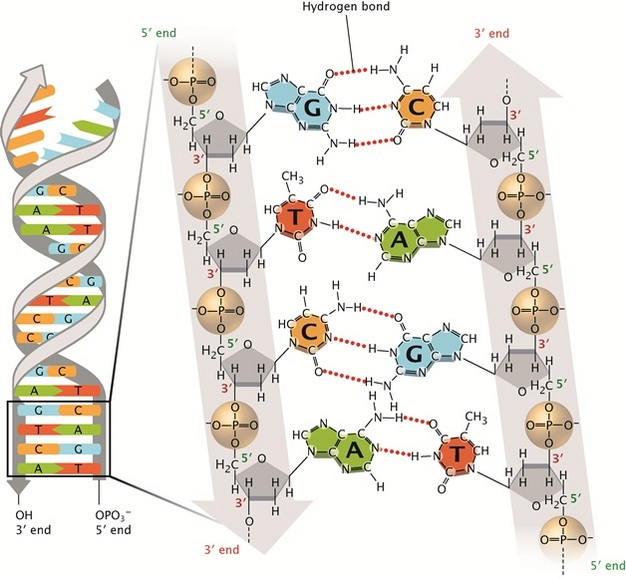
\includegraphics[width=12cm]{images/double_helix.jpg}
    \caption[DNA double helix]{DNA double helix base pairing \cite{pray2008discovery}.}
    \label{fig:double_helix}
\end{figure}

In DNA sequence analysis, it often makes sense to refer to a subsequence of a fixed length \(k\). Such subsequence we call a \textbf{k-mer}.

\section{A Brief Overview of Nanopore Sequencing}
Throughout the years, several methods based on different principles have been developed for DNA sequencing, with origins dating back to late $1970$s.  \cite{ambardar2016high}.

The technology of nanopore sequencing is based on the idea of having a two chambers of electrolytic solution separated by an electrically resistant membrane. In the membrane there is a small pore of a diameter approximately $1$ nm (\textbf{n}ano\textbf{m}eter), hence the name nanopore sequencing. Nanopore sequencing devides usually have several hundreds of nanopores in the membrane \cite{ambardar2016high}.

A difference in voltage between the two chambers causes a ionic current to flow from the DNA containing chamber to the the other. A motor protein on one end of each DNA strand attracts it to the nanopore entrance and the strand starts flowing through the nanopore. The current at the nanopore is measured at a fixed sampling frequency that creates a signal. The values of the current depend on the nucleobase flowing through the nanopore, as well as $\approx 5$ previous bases. We can assume that the measured signal id dependent on the actual $6$-mer. The signal measured in the nanopore during sequencing is widely known as \textbf{squiggle}. Squiggles are then subjected to a process which translates them into a DNA sequence of nucleobases - this process is called \textbf{basecalling}.

Nanopore sequencing technology is the third generation sequencing technology that enables sequencing of a much longer reads (up to megabase-long reads) than previous, second generation methods ($150$ bp), while retaining similar low cost. Longer read length is especially useful for biologists as it eliminates the effects of amplification artifacts and PCR bias, but is more prone to errors - the current is erroneous by $\approx 10\%$.


\section{Utilization of Multiplexing}
Flow cells are usually designed for a single sequencing run of $48$ hours' duration. Their reusability is not very straightforward, even though they can be washed with available washing kits\footnote{\url{https://store.nanoporetech.com/eu/flow-cell-wash-kit-r9.html}}, their quality still suffers a noticeable drop down. The sample from previous runs can still be present, contaminating the subsequent runs \cite{storeONT}. It is therefore economically convenient to perform multiple sequencing experiments in a single sequencer run.
This is done by pooling several DNA sequences into one large sample (multiplexing), sequencing the sample in a single run, and then sorting the reads by their origin sequence (demultiplexing).

\begin{figure}[!ht]
    \centering
    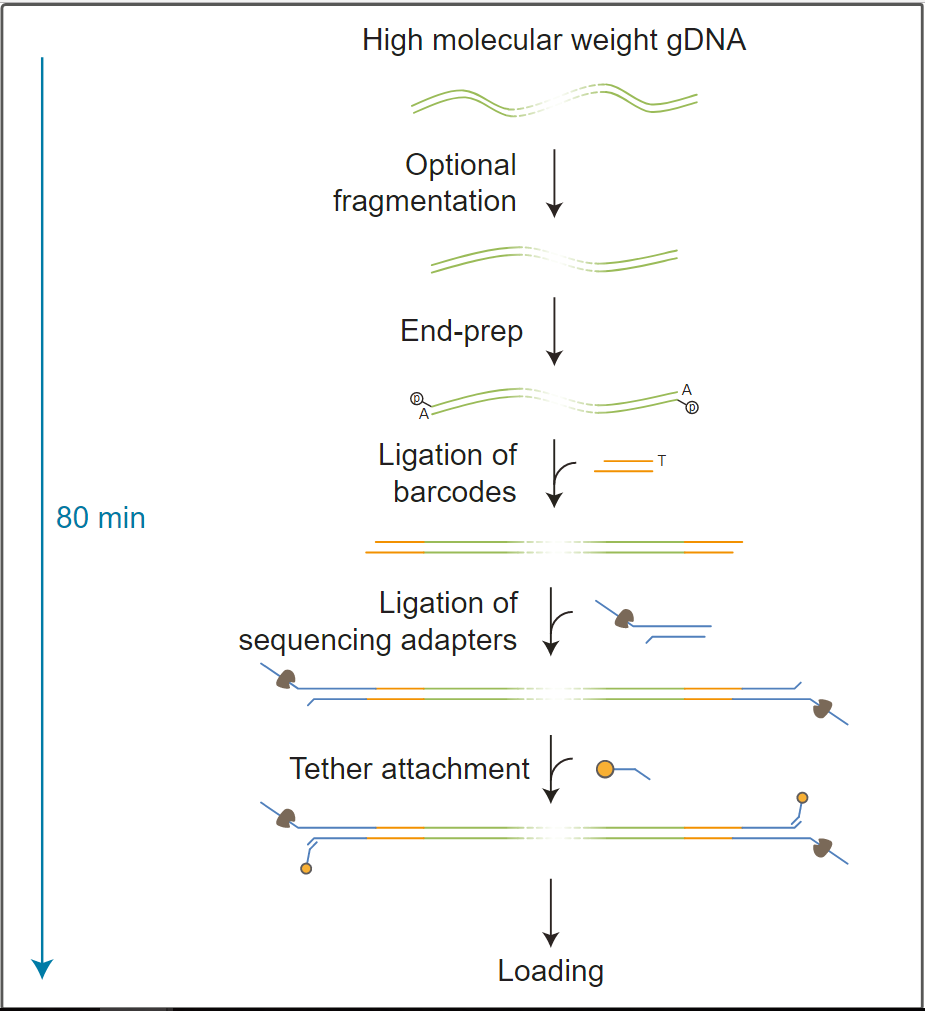
\includegraphics[scale=0.7]{images/barcoding.png}
    \caption[Sequencing preparation workflow.]{Sequencing preparation workflow with the use of Native Barcoding Kit as documented by Oxford Nanopore Technologies \cite{BarcodesONT}.}
    \label{fig:barcodes_workflow}
\end{figure}

To perform demultiplexing (sometimes also called deconvolution) step, reads need to be labeled uniquely in accordance to their origin sequence. This task is carried out by so-called \textit{barcodes} - short DNA sequences inserted to pooled fragments by an enzymatic process called \textit{ligation}, that uniquely determine their origin. The barcoding workflow is presented in Fig. \ref{fig:barcodes_workflow}.  Barcodes are prepared beforehand in kits, in which each barcode material is located in a tube. Barcodes are designed so that they to minimize cross-talk \cite{BarcodesONT}.

However, as nanopore sequencing produces erroneous signals, these errors may also occur within the barcodes, which significantly complicates the process of demultiplexing, often resulting in inability to determine the origin of a fragment and thus losing it for further analysis. We can look at the process of sorting the reads according to their barcode label as a clustering problem.

\section{Demultiplexing Techniques}
Several different methods have been developed for the process of demultiplexing in third generation sequencing. We provide a brief overview of their characteristic features as well as a notion of their performance.

\subsection{Albacore}
Albacore is a proprietary tool developed by Oxford Nanopore Technologies. Its main capability is basecalling with the use of recurrent neural networks, though it also supports barcode demultiplexing for several barcoding kits from ONT library. Albacore first basecalls the reads and subsequently tries to identify the barcodes by alignment of the barcode sequences to the basecalled read. Typically, Albacore can classify reads with an accuracy of $\approx 97\%$ \cite{Deepbinner}, but fails to assign a barcode label to $\approx 20\%$, meaning that $\frac{1}{5}$ of all sequenced reads will be unusable for following analyses \cite{Deepbinner}.

\subsection{Porechop}
Porechop is a tool developed by Ryan R. Wick, primarily designed for finding and removing adapters, but also supports demultiplexiing of reads barcoded by ONT barcoding kits \cite{Porechop}. Porechop operates on basecalled sequences in a similar manner to Albacore, by aligning the searched sequences and comparing the score with a pre-defined treshold. When used jointly with Albacore, the chance for misclassification of reads can be minimized \cite{Porechop}. Porechop remains unmaintained since October $2018$.

\subsection{Deepbinner}
Another demultiplexing tool called \textbf{Deepbinner}, developed by Ryan R. Wick et al. \cite{Deepbinner}, uses a deep convolutional neural network (CNN) to classify reads. CNNs are widely used in image processing domain for tasks like object localization, classification, etc. In contrast with Albacore and Porechop, Deepbinner takes raw sequencing squiggle as an input, which eliminates the errors made by  basecalling. The CNN is trained on the specific barcode set in a supervised manner, which means that a large number of squiggles is required, preferably from multiple sequencing runs \cite{Deepbinner}.

\begin{figure}
    \centering
    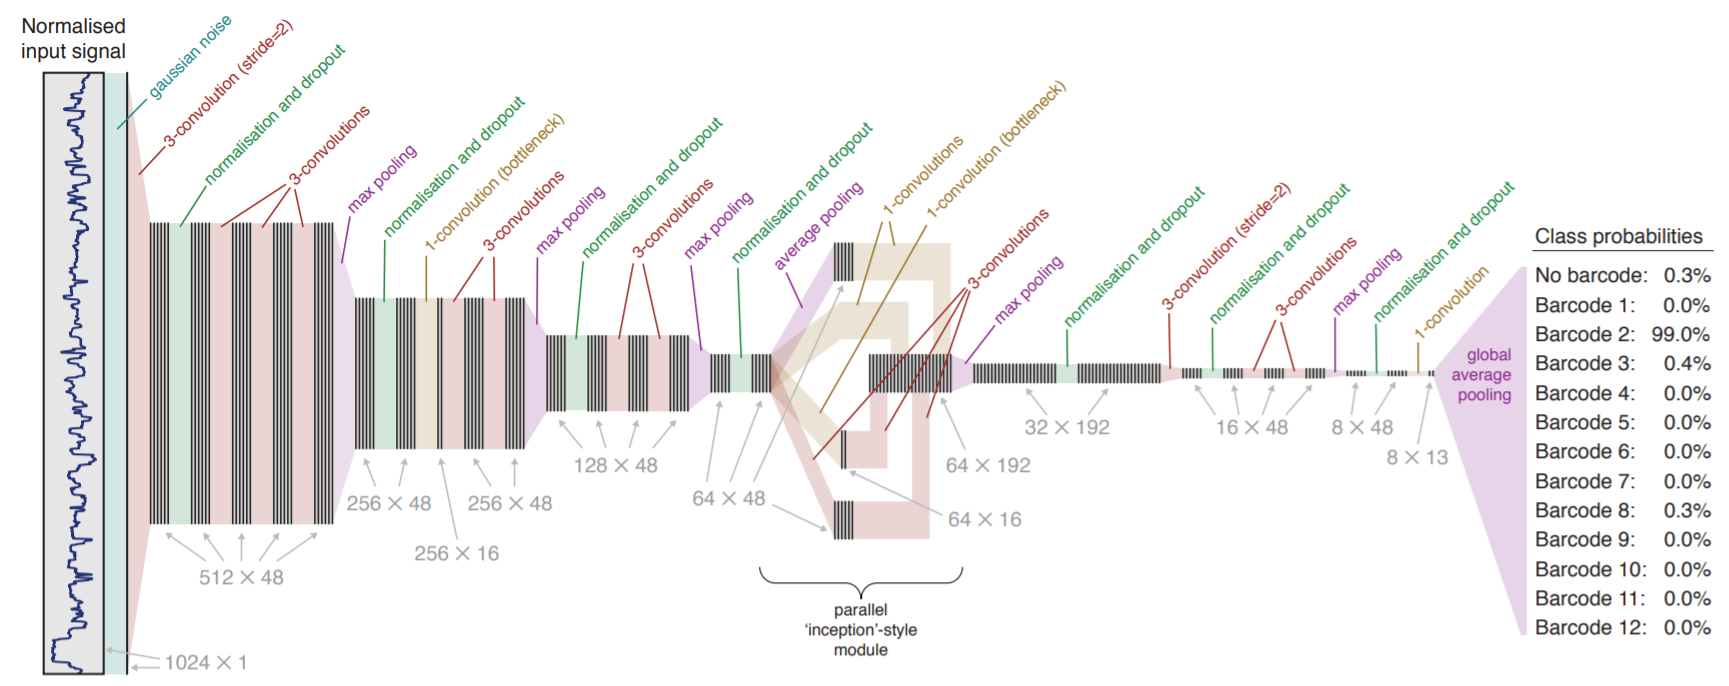
\includegraphics[width=\textwidth]{images/deepbinner_cnn.png}
    \caption[Deepbinner's CNN architecture]{The architecture of the Deepbinner's convolutional neural network \cite{Deepbinner}.}
    \label{fig:deepbinner_cnn}
\end{figure}

Deepbinner assigns a barcode label to $93.33\%$ of all reads, while its accuracy on the binned reads reaches as much as $98.41\%$ \cite{Deepbinner}, which makes it superior to both Albacore and Porechop.

\subsubsection{Using more demultiplexers jointly}
Apart from using a single demultiplexing tool it is also possible to use two at once, e.g. using one to validate the other. Wick et al. examined usage of Deepbinner jointly with Albacore and Albacore jointly with Porechop binning only reads on which both demultiplexers agree on labels. This improved the overall precision, but at the cost of rendering more reads unlabeled \cite{Deepbinner}.